\documentclass[12pt]{article}
\usepackage{graphicx} % Required for inserting images
\usepackage{mathtools}
\usepackage{amsmath}
\usepackage{gvv-book}
\usepackage{gvv}
\usepackage[shortlabels]{enumitem}
\usepackage{multicol}

\title{\textbf{12.122}}
\author{\textbf{EE25BTECH11004 - Aditya Appana}}
\date{October 9, 2025}
\renewcommand{\labelenumi}{\Alph{enumi})}
\begin{document}

\maketitle

\section*{Question}
The $S_2$ operation on a molecule with the axis of rotation as the Z-axis, moves a nucleus at $(x,y,z)$ to
\begin{enumerate}
\begin{multicols}{4}
    \item $(-x,-y,z)$
    \item $(x,-y,-z)$
    \item $(-x,y,-z)$
    \item $(-x,-y,-z)$
\end{multicols}
\end{enumerate}
\section*{Solution}

The rotation matrix for a rotation by an angle $\theta$ about the z-axis is:
\begin{align}
R_z(\theta) = \myvec{
\cos\theta & -\sin\theta & 0 \\
\sin\theta & \cos\theta & 0 \\
0 & 0 & 1}
\end{align}\\
Let the point be $\vec{x} = \myvec{x\\y\\z}$. Therefore the rotated vector will be:
\begin{align}
 R_z(\theta)\vec{x} =
 \myvec{\cos\theta & -\sin\theta & 0 \\\sin\theta & \cos\theta & 0 \\0 & 0 & 1}\myvec{x\\y\\z}\\
 \myvec{x\cos\theta - y\sin\theta \\ x\sin\theta +y\cos\theta \\ z}
\end{align}\\
It can be seen that a rotation about the Z-axis does not change the z-coordinate. Hence option(\textbf{A}) is correct.

\begin{figure}[H]
    \centering
    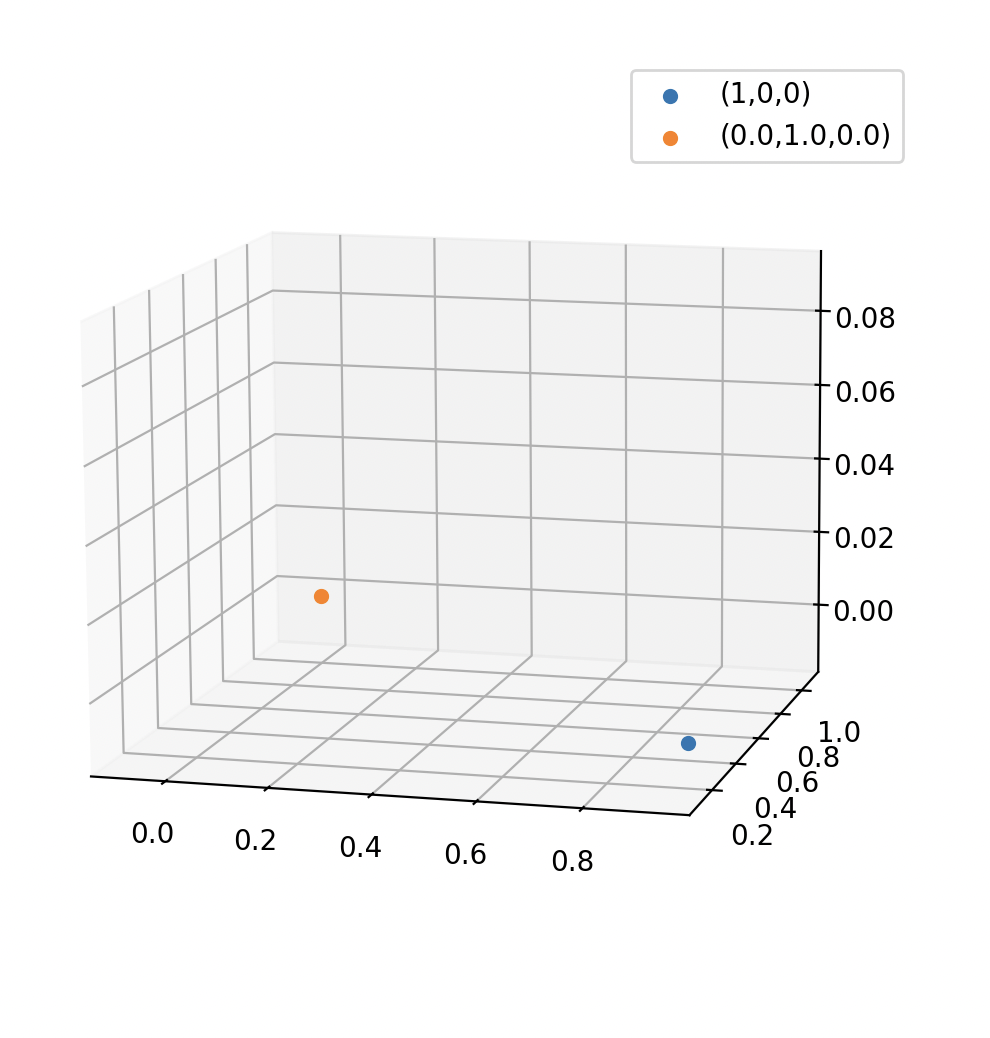
\includegraphics[width=0.8\columnwidth]{Figs/12122.png}
    \caption{Plot}
    \label{fig:placeholder}
\end{figure}
\end{document}
